\documentclass{letter}

\usepackage[left=0.75in, right=0.75in, top=1.1in, bottom=0.75in]{geometry}
\usepackage{fancyhdr, amsmath, amssymb, mathtools, xcolor, graphicx, listings, mathpazo, xfrac}
\graphicspath{{.}}

\pagestyle{fancy}
\fancyhf{}
\rhead{Page \thepage}
\chead{AMSC808N Final Exam Problem 1}
\lhead{Tyler Hoffman}
\setlength{\headsep}{0.2in}

\newcounter{problem}
\newcounter{subproblem}[problem]
\newcounter{solution}

\renewcommand{\thesubproblem}{(\alph{subproblem})}

\newcommand{\Problem}[2]{%
	\stepcounter{problem}%
	\leftskip=0pt%
	\theproblem.~\textbf{{#1.}} #2 \par%
}

\newcommand{\Subproblem}[1]{%
	\stepcounter{subproblem}%
	\leftskip=15pt%
	\thesubproblem~ #1 \par%
}

\newcommand{\Solution}[1]{%
	\textbf{Solution.} #1 \par%
}

\newcommand{\Due}[1]{\textbf{Due: #1} \par}

\newcommand{\UNFINISHED}{\textbf{\color{red} UNFINISHED}}
\newcommand{\CHECK}{\textbf{\color{orange} CHECK ME}}

\newcommand{\iu}{{i\mkern1mu}}
\newcommand{\T}{\intercal}
\newcommand{\R}{\mathbb{R}}
\newcommand{\relu}{\mathrm{ReLU}}

\DeclareMathOperator{\diag}{diag}
\DeclareMathOperator{\rank}{rank}
\DeclareMathOperator{\nul}{nul}
\DeclareMathOperator{\tr}{tr}

\usepackage{hyperref}
\begin{document}
    \Due{21 Dec 2020}

    The code for this problem can be found at \href{https://github.com/thoffman1/amsc808n/tree/master/final/problem1}{this Github link}.

    Suppose we want to approximate the function $g(x) = 1 - \cos(x)$ on the interval $[0, \pi/2]$ with the function $\relu(ax - b)$ where $a$ and $b$ are to be determined. We take 6 training points $x_j = \pi j/10$, $j = 0,1,2,3,4,5$ and set up the following loss function: \begin{align*}
        f(a, b) = \frac{1}{12}\sum_{j = 0}^5 [\relu(ax_j - b) - g(x_j)]^2.
    \end{align*}

    \Problem{Stationary points}{The set of stationary points of $f$ (i.e., the set of points where $\nabla f = 0$) consists of the global minimizer and a flat region. Describe this set analytically using equalities and inequalities and show it in a figure. Provide an analytic formula for the global minimizer of $f$. What is the global minimum of $f$?}
    \Solution{To begin, we compute the partial derivatives of $f$. \begin{align*}
        \frac{\partial f}{\partial a} &= \frac{1}{6}\sum_{j = 0}^5 x_j[\relu(ax_j - b) - g(x_j)]\relu'(ax_j - b) \\
        \frac{\partial f}{\partial b} &= -\frac{1}{6}\sum_{j = 0}^5 [\relu(ax_j - b) - g(x_j)]\relu'(ax_j - b)
    \end{align*} where the derivative of the $\relu$ is defined as \begin{align*}
        \relu'(x) = \begin{cases} 1 & x > 0 \\ 0 & x < 0. \end{cases}
    \end{align*} In order to guarantee that the partials are equal to 0, we look for values of $a$ and $b$ that make the terms in the interior equal to 0. First, we study the $\relu'$ factor and notice that \begin{align*}
        \relu'(ax_j - b) = 0 \iff ax_j - b < 0
    \end{align*} so $b > ax_j$ for all $j$ in order to zero out every term in both sums. Since $x_0 = 0$, we know $b > 0$. When $a > 0$, we need $b > \max_j ax_j = \frac{\pi}{2}a$ and when $a < 0$, we need $b > \min_j ax_j = 0$ since the inequality flips when $a < 0$. Naturally, when $a = 0$ we simply need $b > 0$ (as $\relu(-b) = 0$ for $b > 0$), which squares up with the above characterization. This flat region can be seen in Figure 1 below. 
    
    \begin{center}
        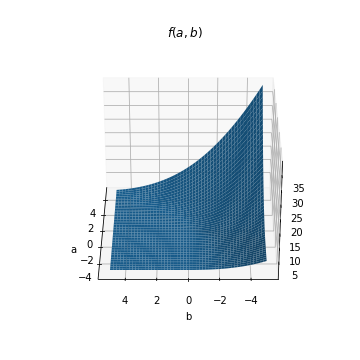
\includegraphics[trim={1cm 1cm 1cm 0cm},clip,scale=0.7]{../pics/loss_surface.png} 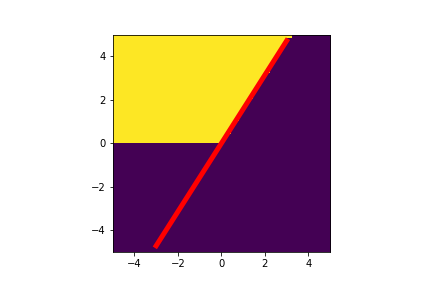
\includegraphics[trim={1cm 0cm 1cm 0cm},clip,scale=0.7]{../pics/flat_region.png}\\
        Figure 1: Left: surface of $f(a, b)$ near the origin. Right: flat region $\nabla f = 0$. The yellow region is the flat region, the purple region is the rest of the function, and the red line is the boundary $b = \frac{\pi}{2}a$.
    \end{center}

    To find the minimizer, we need to consider other parts of the terms in the sum---finding where the $\relu'$ factors are zero only gives us information about the flat region. We examine the $\relu(ax_j - b) - g(x_j)$ factor and think about where it zeros out: \begin{align*}
        0 = \relu\left(\frac{\pi j}{10}a - b\right) - 1 + \cos\left(\frac{\pi j}{10}\right) &= \max\left(0, \frac{\pi j}{10}a - b\right) - 1 + \cos\left(\frac{\pi j}{10}\right) \\
        \implies \max\left(0, \frac{\pi j}{10}a - b\right) &= 1 - \cos\left(\frac{\pi j}{10}\right) \, \, \forall j = 0, 1, 2, 3, 4, 5.
    \end{align*} For $j = 0$, we get the equation $\max(0, -b) = 0$ which implies that $b > 0$. For all the other $j$, we can drop the $\max$ on the left-hand side because the right-hand side is greater than 0, so we know the left-hand side will need to similarly be positive. Plugging in the rest of the $j$ gives the following system of equations: \begin{align*}
            \frac{\pi}{10}a - b &= 1 - \cos\left(\frac{\pi}{10}\right) \\
            \frac{\pi}{5}a - b &= 1 - \cos\left(\frac{\pi}{5}\right) \\
            \frac{3\pi}{10}a - b &= 1 - \cos\left(\frac{3\pi}{10}\right) \\
            \frac{2\pi}{5}a - b &= 1 - \cos\left(\frac{2\pi}{5}\right) \\
            \frac{\pi}{2}a - b &= 1 - \cos\left(\frac{\pi}{2}\right) 
    \end{align*} which can be written as the matrix equation $Cx = d$ where \begin{align*}
        C = \begin{bmatrix} \sfrac{\pi}{10} & -1 \\
            \sfrac{\pi}{5} & -1 \\
            \sfrac{3\pi}{10} & -1 \\
            \sfrac{2\pi}{5} & -1 \\
            \sfrac{\pi}{2} & -1 \\
        \end{bmatrix}, x = \begin{bmatrix} a \\ b \end{bmatrix}, \text{ and }
        d = \begin{bmatrix}  
            1 - \cos\left(\sfrac{\pi}{10}\right) \\ 
            1 - \cos\left(\sfrac{\pi}{5}\right) \\ 
            1 - \cos\left(\sfrac{3\pi}{10}\right) \\ 
            1 - \cos\left(\sfrac{2\pi}{5}\right) \\ 
            1 - \cos\left(\sfrac{\pi}{2}\right) 
        \end{bmatrix}.
    \end{align*} So we could say that the minimizer $x^*$ is the solution of this system $x^* = C^{-1}d$. However, this system is overdetermined and is not guaranteed to have a nice, unique solution. This is because we are not taking into account the $\relu'$ terms, which will turn on and off certain rows of the left-hand side based on whether or not the argument is negative, something which will be important in the minimizer. To incorporate this, we multiply both sides by the vector $y(a,b)$: \begin{align*} 
        y(a, b) = \begin{bmatrix} 
            \relu'\left(\sfrac{\pi a}{10} - b\right) \\
            \relu'\left(\sfrac{\pi a}{5} - b\right) \\
            \relu'\left(\sfrac{3\pi a}{10} - b\right) \\
            \relu'\left(\sfrac{2\pi a}{5} - b\right) \\
            \relu'\left(\sfrac{\pi a}{2} - b\right)
        \end{bmatrix}    
    \end{align*} which turns this into the nonlinear system $(y \odot C)x = y \odot d$. The minimizer will then be the solution $x^* = (y \odot C)^{-1}(y \odot d)$, which can be computed as $x^* = [0.86128902, 0.37349155]$ by solving this system (see code for details). Here, $\odot$ denotes the entry-wise (Hadamard product).}
    \pagebreak
    \Problem{Gradient descent}{Take $a = 1$ and $b = 0$ as the initial guess for gradient descent with constant stepsize. What is the minimal stepsize $\alpha^*$ such that the iterates end up in the flat region? Suppose we take $\alpha = 0.99\alpha^*$ and run gradient descent. Will the iterates approach the global minimizer? Either way, explain why. Propose a stepsize trying to make it as large as possible such that the iterates will necessarily converge to the global minimizer and give a rationale for your choice.}
    \Solution{The gradient descent iteration is $x_{k+1} = x_k - \alpha \nabla f(x_k)$. Here, $x = [a, b]^\T \in \R^2$. See Figure 2 below for an illustration of the first step of gradient descent when run from $x_0 = [1, 0]$. The minimal step size $\alpha^*$ will be the step size that causes us to step over the blue line $b = \frac{\pi}{2}a$ and remain in the flat region for all future iterations. The slope of this orange line is \begin{align*}
        m = \frac{[\nabla f(1,0)]_2 - 0}{1 + [\nabla f(1,0)]_1 - 1} = \frac{[\nabla f(1,0)]_2}{[\nabla f(1,0)]_1}
    \end{align*} where $[\cdot]_i$ indicates the $i$th component of that vector. Hence the orange line has equation $b = m(a-1)$ and we seek its intersection with the line $b = \frac{\pi}{2}a$ by solving the system: \begin{align*}
        \begin{cases}
            ma - b = m \\
            \frac{\pi}{2}a - b = 0
        \end{cases}
    \end{align*} which gives the intersection point $(\hat{a}, \hat{b}) = (0.37958407, 0.59624926)$ and thus the distance from the intersection to the initial point is $d = \sqrt{(\hat{a} - 1)^2 + \hat{b}^2} = 0.8604819$. Therefore, the minimal step size $\alpha^*$ such that we end up in the flat region is the value such that $\|\nabla f(1, 0)\|\alpha = d$, implying that $\alpha^* = \sfrac{d}{\|\nabla f(1, 0)\|} = 1.50996024102$. 
    
    If we take $\alpha = 0.99\alpha^*$ and run gradient descent, the iterates will approach the global minimizer but slowly and never quite get there. They do not make it out of the neighborhood of the minimizer, but rather alternate between sides of this neighborhood as the gradient very slowly decays. All of my numerical tests using $\alpha = 0.99\alpha^*$ resulted in the method taking around $10^6$ iterations to converge and even then it never exactly hit the minimizer since it relied on the gradient being small enough to carry it there, which didn't happen. 
    
    As for the largest possible step size, it must be small enough that the iterates will reach the minimizer at the very end of the iteration. I ran experiments for a number of values of $\alpha$ and examined if they hit the flat region or not. If the gradient descent iteration hit 1000 iterations (far more than any of the convergent experiments), then I stopped it early and recorded that value of $\alpha$ as hitting the flat region. Figure 3 shows this plot, where the $y$ axis is 1 if the cutoff was reached and 0 otherwise. In this sweep, the largest value of $\alpha$ that does not hit the cutoff is $\alpha = 1.30476051596$, so it is my answer for the largest possible step size where the iterates still converge to the global minimizer.
    \begin{center}
        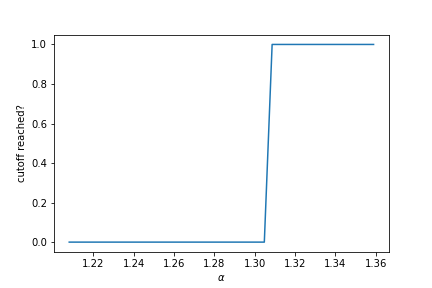
\includegraphics[scale=0.77]{../pics/cutoffs.png} \\
        Figure 3: Stepsizes and if they hit the flat region for $\alpha = p\alpha^*$ for 40 values of $p$ between 0.8 and 0.9. 
    \end{center}

    \begin{center}
        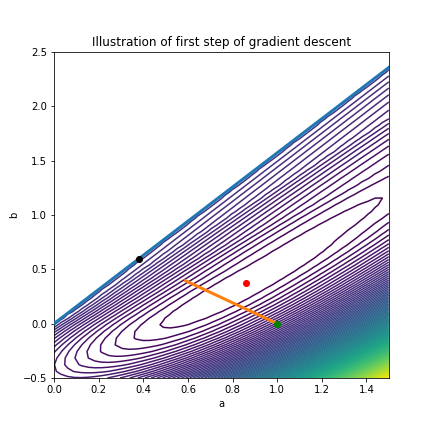
\includegraphics{../pics/gd_firststep.png} \\
        Figure 2: Illustration of the first step of gradient descent. Green dot is the initial point $x_0 = [1, 0]$, red dot is the global minimizer $x^*$, the black dot is the intersection between the gradient line and the blue line, the blue line is the line $b = \frac{\pi}{2}a$, the orange line is the vector $\nabla f(1, 0)$, and the contours are the contours of the function $f(a, b)$.
    \end{center}}

    \Problem{Stochastic gradient descent}{As above, take $a = 1$ and $b = 0$ as the initial guess. Use a simple stochastic gradient descent with a single training point chosen randomly for approximating the gradient of $f$ at each step. Find a strategy for stepsize reduction such that the stochastic gradient descent will converge to the global minimizer.}
    \Solution{See \texttt{prob1.ipynb} for my stochastic gradient descent code. I tested the following schedules: \begin{itemize}
        \item Reciprocal: $\alpha_k = L/k$
        \item Power: $\alpha_k = L2^{-k-1}$
        \item Exponential $\alpha_k = Le^{-rk}$ where $r$ controls the speed of the decay
        \item Drop: $\alpha_k = Lr^{\lfloor k/M \rfloor}$ where $M$ is the number of steps we take per drop
    \end{itemize} In all of these, $L$ is a constant initial learning rate. These all satisfy $\sum_{k=0}^\infty \alpha_k = \infty$, $\sum_{k=0}^\infty \alpha_k^2 < \infty$. Moreover, they all worked, just at different rates of convergence. \UNFINISHED}
\end{document}